\chapter{Arm Length Compensation System}





\section{Basics in Vibration Isolation System}
Basics of the vibration isolation system for GW detectors is the multiple-stage pendulum with low resonance frequency, which is the passive vibration isolation. Actually, in order to improve the bandwidth of the viblation isolation, we use some additional sensor to decopule the suspension from the seismic noise, which is the active vibration isolation.

\subsection{Passive Vibration Isolation}
A pendulum works as a mechanical filter attenuating the seismic noise, and it realizes the passive vibration isolation system.

\subsubsection{Single Pendulum}
For simple example, as shown in left figure in Fig.(\ref{img:img501}), consider a one-dimentional harmonic oscillator consisting of a spring with a spring constant $k$ and mass $M$. The displacement of the suspension point and the mass are $x_0$ and $x$, respectively. Because the equation of the motion is written as
\begin{eqnarray} \label{eq:eq501}
  M\ddot{x} = -k(x-x_0),
\end{eqnarray}
the frequency transfer function from the displacement of the suspension point to the mass displacement $H(f)$ is given by the Fourier transform from the equation and represented as
\begin{eqnarray} \label{eq:eq502}
  H(f) \equiv \frac{1}{1-(f/f_0)^2},
\end{eqnarray}
where $f_0 = (k/M)^{1/2}$ is the resonant angular frequency of the oscillator.

According to Eq.(\ref{eq:eq502}), the amplitude of $H(f)$ is unity below the resonant frequency, the amplitude is approximately propotional to $(f/f_0)^{-2}$ above resonance frequency. The bode plot of $H(f)$ with various resonance frequencies are plotted in right figure in Fig. \ref{img:img501} . One finds that it is better to make a low-resonance frequency oscillator in order to attenuate the seismic noise broadly. 

\begin{figure}[h]
  \begin{center}   
    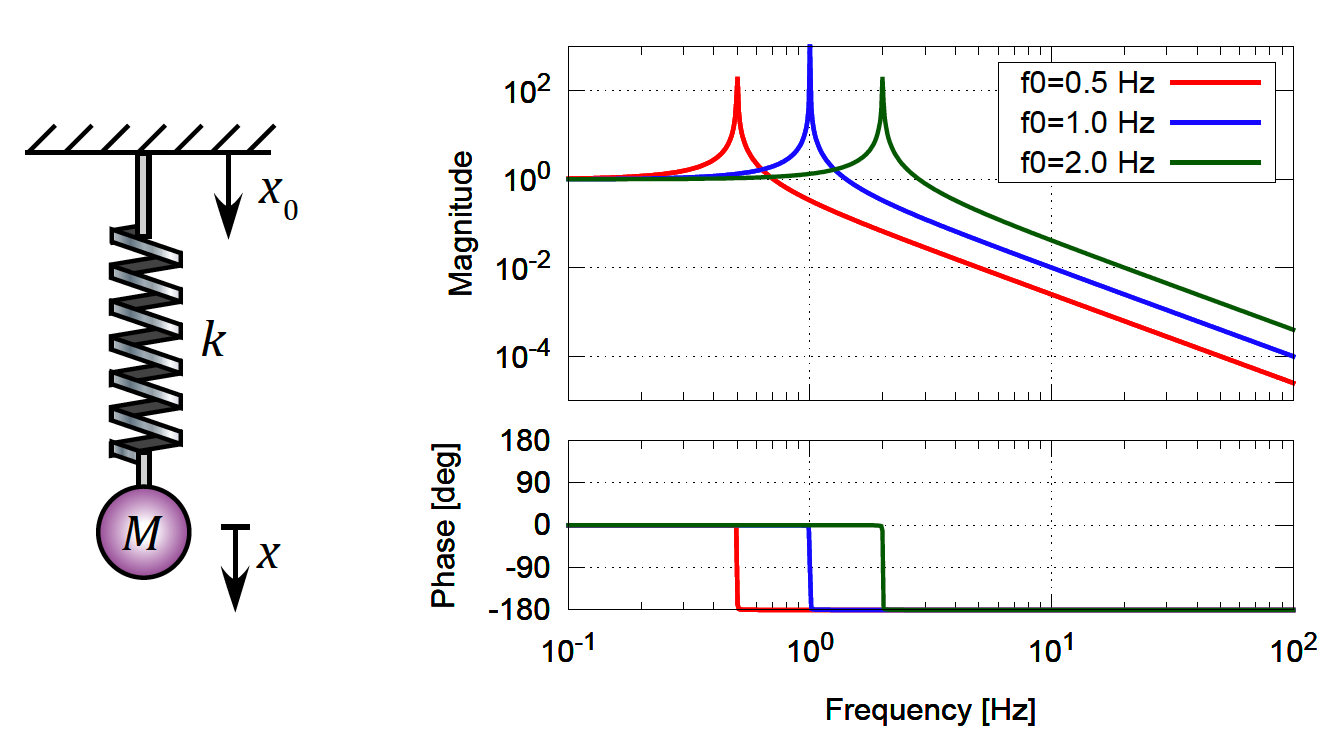
\includegraphics[width=11cm,height=6cm]{./img_chap5/img501.png}
    \caption{Single pendulum as a mechanical filter and its transfer function with various resonant frequencies. This figure is cited from Fig.(2.3) in \cite{sekiguchi2016astudy}.} \label{img:img501}
  \end{center}
\end{figure}

\subsubsection{Multi-stage Pendulum}
In order to increase the order of the seismic isolation, multi-stage pendulum is effective. In case of an N-stage pendulum, the transfer function from the ground to the suspended mass is propotional to $f^{-2N}$ above the resonance frequrncy of the pendulum as shown in Fig. \ref{img:img502}. 
\begin{figure}[h]
  \begin{center}   
    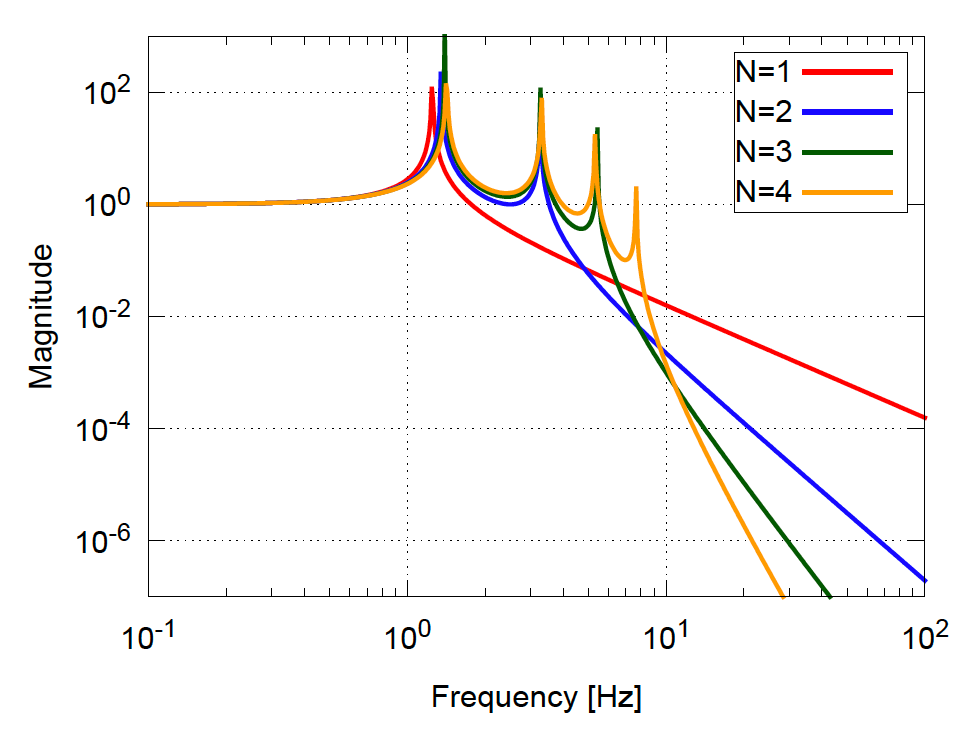
\includegraphics[width=11cm]{./img_chap5/img502.png}
    \caption{The amplitude of the transfer function of the N-stage pendulum. This figure is cited from Fig. 2.4 in \cite{sekiguchi2016astudy}.} \label{img:img502}
  \end{center}
\end{figure}

\subsection{Active Vibration Isolation}
\begin{figure}[h]
  \begin{center}   
    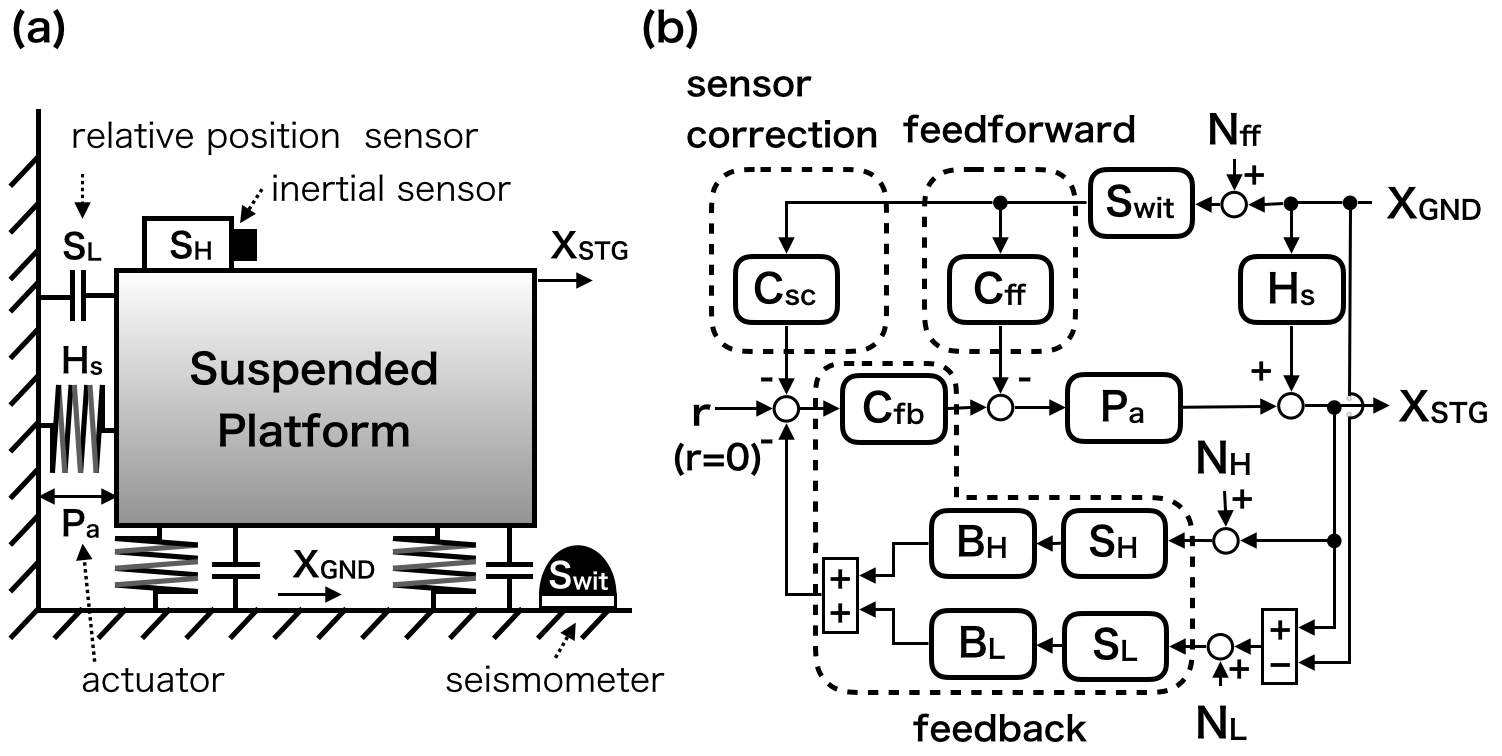
\includegraphics[width=13.5cm]{./img_chap5/img503.png}
    \caption{{\bf(a)} Schematic drawing of an active vibration isolation system for platform. {\bf(b)} Block diagram of the active control scheme.} \label{img:img503}
  \end{center}
\end{figure}

Actual seismic isolation systems use the passive-active concept \cite{matichard2015seismic}. While the passive isolation can attenuate the seismic noise above the resonance frequency, the low-frequency seismic noise below that cannot. In order to compensate for this limitation in low frequency, the active seismic isolation platform is used.

The active isolation system is shown in Fig. \ref{img:img503}(a). A platform is suspended from the ground with transmisivity $H_{\mathrm{s}}$. This platfrom is fed back both signal of a inertial sensor with calibration factor $S_{\mathrm{H}}$ and signal of a relative position sensor with calibration factor $S_{\mathrm{L}}$, to the platform using actuator with actuator efficiency $P_{\mathrm{a}}$. This feedback control actively decouple the platform from the seismic disturbance from $0.1\,\mathrm{Hz}$ to a few Hz. Moreover, the platform is controled with feedforward using a seismometer with calibration factor $S_{\mathrm{ff}}$ installed on the local ground. 

能動防振の制御方法はFig.\ref{img:img503}(b)に示しているとおり、フィードバック制御、センサーコレクション制御、フィードフォワード制御、が組み合わされている。順番にそれらを説明する。

\subsubsection{feedback control}
制御信号には慣性センサーと相対位置センサーをブレンドして使う。慣性センサーは低周波で感度が悪くなるので慣性センサーにはハイパスフィルター$B_{\mathrm{H}}$をかけ、これに対して相対位置センサーには、
\begin{eqnarray}
  B_{\mathrm{H}}S_{\mathrm{H}} + B_{\mathrm{L}}S_{\mathrm{L}} = 1   \label{eq:eq506}
\end{eqnarray}
となるような相補的なローパスフィルター$B_{\mathrm{L}}$をかける。

このようにブレンドされた制御信号をつかってフィードバック制御した場合での、プラットフォームのステージの変位を考える。まず、platform のステージの変位 $X_{\mathrm{STG}}$は地面振動$X_{\mathrm{GND}}$、慣性センサーノイズ$N_{\mathrm{H}}$、相対位置センサーのノイズ$N_{\mathrm{H}}$で表すと
\begin{eqnarray}
  \label{eq:eq510}
  X_{\mathrm{STG}} = \frac{G}{1+G}LX_{\mathrm{GND}} + \frac{1}{1+G}H_{\mathrm{s}}X_{\mathrm{GND}} + \frac{G}{1+G}\left(HN_{H}+LN_{L}\right)
\end{eqnarray}
のようになる。ここで、ループゲインを$G=C_{\mathrm{fb}}P_{\mathrm{a}}$、相補フィルターとそれぞれのセンサー効率の積を$L=B_{\mathrm{H}}S_{\mathrm{H}}$、$H=B_{\mathrm{L}}S_{\mathrm{L}}$として、さらに計算の途中でEq.(\ref{eq:eq506})をつかった。すなわち、フィードバック制御が十分に働いている場合、つまりループゲインの値が十分に大きいときのステージの変位は
\begin{eqnarray}
  \lim_{G\to\infty} X_{\mathrm{STG}} = LX_{\mathrm{GND}} + \left(HN_{H}+LN_{L}\right) \label{eq:eq510_a}
\end{eqnarray}
である。

Eq.(\ref{eq:eq510_a})によれば、ステージの変位を慣性系に対して防振させるためには伝達関数$L$を小さくすればよいが、これは同時に相補フィルターである$H$を大きくすることを意味し、かえって慣性センサーのノイズをステージに流入させてしまう。現実的には、ローパスフィルター$B_{\mathrm{L}}$のカットオフ周波数は$100\,\mathrm{mHz}$が限界であり、それ以下の周波数では地面振動は防振されない。別の言い方をすれば、慣性センサーをつかったフィードバック制御は、ブレンディングフィルター$L$で地面振動からステージへの応答を整えることができる一方で、低周波の感度不足によって防振できる帯域が制限される。



\subsubsection{Sensor Correction Technique}
センサーコレクション制御は、地面においた感度の良い別の慣性センサーで、フィードバック用の慣性センサーの感度不足を補う制御である。Eq.(\ref{eq:eq506})の関係をもつ相補フィルターでブレンドされた制御信号をつかうと、慣性センサーの感度が足りない低周波帯域では、相対位置センサーの信号をつかってフィードバック制御をしなければならない。この相対位置センサーは地面からのステージの変位を測るので、低周波帯域では、ステージは地面に対して同じに動くことを意味する。センサーコレクション制御は、もう一つの地震計で測定した地面振動をつかって、この制御信号から地面振動を取り除くことで、制御信号を慣性系からみたステージの変位信号に補正する。



\begin{eqnarray}\nonumber
  X_{\mathrm{STG}} &=&\frac{G}{1+G}L\left(1-C_{\mathrm{sc}}\frac{S_{\mathrm{ff}}}{L}\right) X_{\mathrm{GND}} + \frac{1}{1+G}H_{\mathrm{s}}X_{\mathrm{GND}}\\ 
  &+& \frac{G}{1+G}\left(HN_{H}+LN_{L}\right) + \frac{G}{1+G}C_{\mathrm{sc}}S_{\mathrm{ff}}N_{\mathrm{ff}}
\end{eqnarray}\label{eq:eq511}

\subsubsection{Feedforward Technique}
\begin{eqnarray}\nonumber
  X_{\mathrm{STG}} &=&\frac{G}{1+G}L\left(1-C_{\mathrm{sc}}\frac{S_{\mathrm{ff}}}{L}\right) X_{\mathrm{GND}} + \frac{1}{1+G}\left(H_{\mathrm{s}}-P_{\mathrm{a}} C_{\mathrm{ff}} S_{\mathrm{ff}}\right) X_{\mathrm{GND}}\\ \nonumber
  &+& \frac{G}{1+G}\left(HN_{H}+LN_{L}\right) + \frac{G}{1+G}C_{\mathrm{sc}}S_{\mathrm{ff}}N_{\mathrm{ff}} \\ 
  &+& \frac{1}{1+G}P_{\mathrm{a}} C_{\mathrm{ff}}S_{\mathrm{ff}}N_{\mathrm{ff}}
\end{eqnarray}\label{eq:eq512}


\subsection{Toward the Global Seismic Control}
\subsubsection{Overview}
\subsubsection{Suspension Point Interferometer}

%
\section{Difficulties in the Global Seismic Control}
\subsection{Overview}
\subsection{Actuator Range Limit}
\subsection{...}
\subsection{...}


%
\section{Arm Length Compensation Using Geophysics Interferometer}
\subsection{Concept}
\subsection{Geophysics Interferometer for Sensing the Arm Length}
\subsection{Arm Length Compensation}
\subsection{Requirements}


\section{Summary of the Chapter}
